% Options for packages loaded elsewhere
\PassOptionsToPackage{unicode}{hyperref}
\PassOptionsToPackage{hyphens}{url}
%
\documentclass[
]{article}
\usepackage{amsmath,amssymb}
\usepackage{lmodern}
\usepackage{iftex}
\ifPDFTeX
  \usepackage[T1]{fontenc}
  \usepackage[utf8]{inputenc}
  \usepackage{textcomp} % provide euro and other symbols
\else % if luatex or xetex
  \usepackage{unicode-math}
  \defaultfontfeatures{Scale=MatchLowercase}
  \defaultfontfeatures[\rmfamily]{Ligatures=TeX,Scale=1}
\fi
% Use upquote if available, for straight quotes in verbatim environments
\IfFileExists{upquote.sty}{\usepackage{upquote}}{}
\IfFileExists{microtype.sty}{% use microtype if available
  \usepackage[]{microtype}
  \UseMicrotypeSet[protrusion]{basicmath} % disable protrusion for tt fonts
}{}
\makeatletter
\@ifundefined{KOMAClassName}{% if non-KOMA class
  \IfFileExists{parskip.sty}{%
    \usepackage{parskip}
  }{% else
    \setlength{\parindent}{0pt}
    \setlength{\parskip}{6pt plus 2pt minus 1pt}}
}{% if KOMA class
  \KOMAoptions{parskip=half}}
\makeatother
\usepackage{xcolor}
\usepackage[margin=1in]{geometry}
\usepackage{graphicx}
\makeatletter
\def\maxwidth{\ifdim\Gin@nat@width>\linewidth\linewidth\else\Gin@nat@width\fi}
\def\maxheight{\ifdim\Gin@nat@height>\textheight\textheight\else\Gin@nat@height\fi}
\makeatother
% Scale images if necessary, so that they will not overflow the page
% margins by default, and it is still possible to overwrite the defaults
% using explicit options in \includegraphics[width, height, ...]{}
\setkeys{Gin}{width=\maxwidth,height=\maxheight,keepaspectratio}
% Set default figure placement to htbp
\makeatletter
\def\fps@figure{htbp}
\makeatother
\setlength{\emergencystretch}{3em} % prevent overfull lines
\providecommand{\tightlist}{%
  \setlength{\itemsep}{0pt}\setlength{\parskip}{0pt}}
\setcounter{secnumdepth}{-\maxdimen} % remove section numbering
\ifLuaTeX
  \usepackage{selnolig}  % disable illegal ligatures
\fi
\IfFileExists{bookmark.sty}{\usepackage{bookmark}}{\usepackage{hyperref}}
\IfFileExists{xurl.sty}{\usepackage{xurl}}{} % add URL line breaks if available
\urlstyle{same} % disable monospaced font for URLs
\hypersetup{
  pdftitle={JSC370 Final Project Report},
  pdfauthor={Evelyn Chou},
  hidelinks,
  pdfcreator={LaTeX via pandoc}}

\title{JSC370 Final Project Report}
\author{Evelyn Chou}
\date{}

\begin{document}
\maketitle

\hypertarget{introduction}{%
\subsection{Introduction}\label{introduction}}

Bike share systems are programs that offer short term bike rentals to
inhabitants of a city, providing a convenient and cheaper alternative to
purchasing a bike for thousands of dollars. Bike Share Toronto,
Toronto's bike share system, offers both one time bike rentals, and
annual memberships for a considerably cheaper alternative to purchasing
a new bike. In a city such as Toronto, where bike thefts are rampant,
they also offer the security of nott having to worry about storing your
bike in a secure location. Bike Share Toronto has over 600 stations
across the city where you can rent and dock bikes. This program is
utilized for a multitude of purposes including commute and leisure.

Toronto's Open Data repository offers monthly data on Bike Share
Toronto's ridership, including variables such as the start and end time
of the rental, the bike dock the rental was from, and so much more. Of
particular interest in this report is the start date of the rental,
which will be used to count the total number of bike rentals in a given
day.

Toronto's Open Data repository also offers data on Bike Share Toronto's
rental stations, including variables such as the station id, station
coordinates (longitude and latitude), types of payments accepted at the
station, and many more that will not be used in this report.

Canada's government website stores data on the historical weather for
all weather stations in Canada. Of particular interest in this report is
the historical daily weather in Toronto's weather station. Weather
variables in this dataset include maximum, minimum, and average daily
temperature (°C), total daily precipitation (mm), and total daily snow
(cm).

This study investigates if weather conditions and temporal factors
influence the number of bike share users on a given day in Toronto. This
investigation will be conducted first with the total daily bike rental
count for all stations, and with the daily bike rental count for each
starting station. By understanding the relationship between weather
factors, temporal factors, and bike share ridership, the city can
understand when maintenance should be performed to avoid inconveniencing
members, and when promotions would be viable.

To do this, I will collect Toronto's Open data repository data on Bike
Share Toronto, and Canada's government on historical daily weather in
Toronto's weather station from January 2020 to December 2022.

Note that in this report, tables or figures may be cut off. See the
website for the well-formatted version of tables and figures.

\hypertarget{data-collection}{%
\subsection{Data Collection}\label{data-collection}}

\hypertarget{bike-share-toronto-ridership}{%
\subsubsection{Bike Share Toronto
Ridership}\label{bike-share-toronto-ridership}}

From the Toronto's Open Data repository, we can obtain the data on Bike
Share Toronto's ridership. On the page, there are several buttons, one
for each year. We inspect the buttons for 2020, 2021, and 2022, and
obtain the links to download the zipped files for each year. Each file
contains twelve csv files, one for each month. Using R, download the
zipped files and unzip them using the \texttt{download.file} and
\texttt{unzip}, then read in the csvs. After reading in the twelve csvs
for each year 2020-2022, ensure that all the variable types are
consistent. Some variables such as the bike id appeared as integers in
one file, and characters in another. Such variables were converted to a
suitable type for consistency. In the case of bike id's, all were
converted to integers. Then, combine the data for each month into one
large dataframe for the bikeshare data using \texttt{bind\_rows}.

Table 1, shown below, depicts the top 5 rows of the combined bikeshare
data. The rows in this dataframe are sorted according to column
``Start.Time'', the starting time of the bike rental.

\begin{table}[!h]

\caption{\label{tab:Table 1 First Five Rows of Bike Share Toronto Ridership Data}Table 1: First Five Rows of Bike Share Toronto Ridership Data}
\centering
\begin{tabular}[t]{r|r|r|l|l|l|l|l|r|l}
\hline
Trip.Id & Trip..Duration & Start.Station.Id & Start.Time & Start.Station.Name & End.Station.Id & End.Time & End.Station.Name & Bike.Id & User.Type\\
\hline
7334128 & 648 & 7003 & 01/01/2020 00:08 & Madison Ave / Bloor St W & 7271 & 01/01/2020 00:19 & Yonge St / Alexander St - SMART & 3104 & Annual Member\\
\hline
7334129 & 419 & 7007 & 01/01/2020 00:10 & College St / Huron St & 7163 & 01/01/2020 00:17 & Yonge St / Wood St & 2126 & Annual Member\\
\hline
7334130 & 566 & 7113 & 01/01/2020 00:13 & Parliament St / Aberdeen Ave & 7108 & 01/01/2020 00:22 & Front St E / Cherry St & 4425 & Annual Member\\
\hline
7334131 & 1274 & 7333 & 01/01/2020 00:17 & King St E / Victoria St & 7311 & 01/01/2020 00:38 & Sherbourne St / Isabella St & 4233 & Annual Member\\
\hline
7334132 & 906 & 7009 & 01/01/2020 00:19 & King St E / Jarvis St & 7004 & 01/01/2020 00:34 & University Ave / Elm St & 2341 & Casual Member\\
\hline
7334133 & 1098 & 7041 & 01/01/2020 00:20 & Edward St / Yonge St & 7134 & 01/01/2020 00:38 & Marlborough Ave / Yonge St & 314 & Annual Member\\
\hline
\end{tabular}
\end{table}

\hypertarget{bike-share-toronto-station}{%
\subsubsection{Bike Share Toronto
Station}\label{bike-share-toronto-station}}

Then we will also obtain the data on Toronto's Bikeshare stations, which
contains the station ids (that correspond to the starting and ending
station id's in the bike ridership data we just downloaded), the
coordinates of the station, and a couple other variables that we will
not be using. To obtain this data, we obtain the links for the json
file, and read in the data using the \texttt{fromJSON} method.

Table 2, shown below, depicts the top 5 rows of the bike station data.

\begin{table}[!h]

\caption{\label{tab:Table 2 First Five Rows of Bike Station Data}Table 2: First Five Rows of Bike Station Data}
\centering
\begin{tabular}[t]{r|r|l|l|l|r|r|r|l|r|l|l|l|l|r|l|l|l|l}
\hline
last\_updated & ttl & data.stations.station\_id & data.stations.name & data.stations.physical\_configuration & data.stations.lat & data.stations.lon & data.stations.altitude & data.stations.address & data.stations.capacity & data.stations.is\_charging\_station & data.stations.rental\_methods & data.stations.groups & data.stations.obcn & data.stations.nearby\_distance & data.stations.\_ride\_code\_support & data.stations.post\_code & data.stations.cross\_street & data.stations.is\_valet\_station\\
\hline
1682364102 & 26 & 7000 & Fort York  Blvd / Capreol Ct & REGULAR & 43.63983 & -79.39595 & 0 & Fort York  Blvd / Capreol Ct & 35 & FALSE & KEY        , TRANSITCARD, CREDITCARD , PHONE &  & 647-643-9607 & 500 & TRUE & NA & NA & NA\\
\hline
1682364102 & 26 & 7001 & Wellesley Station Green P & ELECTRICBIKESTATION & 43.66496 & -79.38355 & 0 & Yonge / Wellesley & 26 & TRUE & KEY        , TRANSITCARD, CREDITCARD , PHONE &  & 416-617-9576 & 500 & TRUE & M4Y 1G7 & NA & NA\\
\hline
1682364102 & 26 & 7002 & St. George St / Bloor St W & REGULAR & 43.66733 & -79.39943 & 0 & St. George St / Bloor St W & 19 & FALSE & KEY        , TRANSITCARD, CREDITCARD , PHONE &  & 647-643-9615 & 500 & TRUE & NA & NA & NA\\
\hline
1682364102 & 26 & 7003 & Madison Ave / Bloor St W & REGULAR & 43.66716 & -79.40276 & NA & Madison Ave / Bloor St W & 15 & FALSE & KEY        , TRANSITCARD, CREDITCARD , PHONE &  & 647-631-4587 & 500 & TRUE & NA & NA & NA\\
\hline
1682364102 & 26 & 7004 & University Ave / Elm St & REGULAR & 43.65652 & -79.38910 & NA & University Ave / Elm St & 11 & FALSE & KEY        , TRANSITCARD, CREDITCARD , PHONE & P7004-7047 & 647-643-9673 & 500 & TRUE & NA & NA & NA\\
\hline
1682364102 & 26 & 7005 & King St W / York St & REGULAR & 43.64800 & -79.38318 & 0 & King St W / York St & 23 & FALSE & KEY        , TRANSITCARD, CREDITCARD , PHONE &  & 647-643-9693 & 500 & TRUE & NA & NA & NA\\
\hline
\end{tabular}
\end{table}

\hypertarget{toronto-weather}{%
\subsubsection{Toronto Weather}\label{toronto-weather}}

From the Canada government webpage, we can access the historical weather
data and select Toronto's weather station. From there, we select the
month and year we wish to obtain. Start with January 2020. The page has
a table with the daily weather data for that month. Inspect the table
and obtain the xml path for it. Then, using R's \texttt{xml2} package,
we can read in the html table. We then convert that table to an R
dataframe using the \texttt{rvest} package. After obtaining the
dataframe for that month, note that the table does not include which
month or year it was from, it only includes the day of the month. Thus,
we add the month and year of the table we just scraped to the dataframe.
Repeat this for all months from January 2020 to December 2022. Finally,
merge all of these dataframes to obtain the combined Toronto weather
data.

Table 3, shown below, shows the first five rows of the combined Toronto
weather data.

\begin{table}[!h]

\caption{\label{tab:Table 3 First Five Rows of Toronto Weather Data}Table 3: First Five Rows of Toronto Weather Data}
\centering
\begin{tabular}[t]{l|l|l|l|l|l|l|l|l|l|l|l|r|r}
\hline
DAY & Max Temp Definition°C & Min Temp Definition°C & Mean Temp Definition°C & Heat Deg Days Definition & Cool Deg Days Definition & Total Rain Definitionmm & Total Snow Definitioncm & Total Precip Definitionmm & Snow on Grnd Definitioncm & Dir of Max Gust Definition10's deg & Spd of Max Gust Definitionkm/h & month & year\\
\hline
01 & 1.0 & -1.2 & -0.1 & 18.1 & 0.0 &  &  & 0.2 & 1 & LegendMM & LegendMM & 1 & 2020\\
\hline
02 & 6.2 & 0.9 & 3.6 & 14.4 & 0.0 &  &  & 0.0 & 1 & LegendMM & LegendMM & 1 & 2020\\
\hline
03 & 7.7 & 3.6 & 5.7 & 12.3 & 0.0 &  &  & 0.0 & 1 & LegendMM & LegendMM & 1 & 2020\\
\hline
04 & 3.6 & 0.3 & 2.0 & 16.0 & 0.0 &  &  & 1.5 & 2 & LegendMM & LegendMM & 1 & 2020\\
\hline
05 & 1.9 & -1.2 & 0.3 & 17.7 & 0.0 &  &  & 5.6 & 2 & LegendMM & LegendMM & 1 & 2020\\
\hline
06 & 2.9 & -1.7 & 0.6 & 17.4 & 0.0 &  &  & 0.2 & 7 & LegendMM & LegendMM & 1 & 2020\\
\hline
\end{tabular}
\end{table}

\hypertarget{data-cleaning-and-wrangling}{%
\subsection{Data Cleaning and
Wrangling}\label{data-cleaning-and-wrangling}}

Tables 1, 2, and 3, from the previous ``Data Collection'' subsection,
provide us with an overview of the data we will be using to answer the
question of interest. However, before that can be done, some data
cleaning and data wrangling needs to be done. We will start with the
bikeshare data.

\hypertarget{bike-share-toronto-ridership-1}{%
\subsubsection{Bike Share Toronto
Ridership}\label{bike-share-toronto-ridership-1}}

We are not actually using most of the variables in the bikeshare data,
we only wish to obtain the number of daily bike rentals. Here we will
create two counts. The number of daily bike rentals for all stations,
and the number of daily bike rentals for each individual starting
station. Thus we will not clean the variables in the bikeshare dataset,
instead we will wrangle the data to obtain our variable of interest:
daily rental count. We will use the start date of each bike rental as
the day it was rented. So if a bike was rented on January 1st, and
returned on January 2nd, we will count this bike in the January 1st
rentals.

To do this, first convert the start date of each rental into a Date
object.

Then, we will count the number of daily bike rentals grouped by the
starting station and save the date, starting station id, and count in a
new dataframe ``count\_station''

Table 4, shown below, shows the first five rows of this new dataframe.
Column ``n'' is the number of bike rentals on that date.

\begin{table}[!h]

\caption{\label{tab:Table 4 First Five Rows of Bikeshare Daily Rental Count}Table 4: First Five Rows of Bikeshare Daily Rental Count}
\centering
\begin{tabular}[t]{r|l|r}
\hline
Start.Station.Id & Date & n\\
\hline
7000 & 2020-01-01 & 4\\
\hline
7000 & 2020-01-02 & 18\\
\hline
7000 & 2020-01-03 & 17\\
\hline
7000 & 2020-01-04 & 16\\
\hline
7000 & 2020-01-05 & 12\\
\hline
7000 & 2020-01-06 & 19\\
\hline
\end{tabular}
\end{table}

\hypertarget{bike-share-toronto-stations}{%
\subsubsection{Bike Share Toronto
Stations}\label{bike-share-toronto-stations}}

Now, we wrangle the data on the bike stations. For this data, we only
have to remove unnecessary variables and rename them for convenience. We
will only keep the station id, name, and the coordinates.

\hypertarget{toronto-weather-1}{%
\subsubsection{Toronto Weather}\label{toronto-weather-1}}

After wrangling the bikeshare and bike station data, we now clean and
wrangle the weather data.

First, consider some rows of the current dataframe. Table 5 below shows
the 101-105th rows of the weather dataframe, which have some problematic
entries.

\begin{table}[!h]

\caption{\label{tab:Table 5 Rows 101-105 of Toronto Weather Data}Table 5: Rows 101-105 of Toronto Weather Data}
\centering
\begin{tabular}[t]{l|l|l|l|l|l|l|l|l|l|l|l|l|r|r}
\hline
  & DAY & Max Temp Definition°C & Min Temp Definition°C & Mean Temp Definition°C & Heat Deg Days Definition & Cool Deg Days Definition & Total Rain Definitionmm & Total Snow Definitioncm & Total Precip Definitionmm & Snow on Grnd Definitioncm & Dir of Max Gust Definition10's deg & Spd of Max Gust Definitionkm/h & month & year\\
\hline
101 & Avg & 7.4 & 0.5 & 4.0 &  &  &  &  &  &  &  &  & 3 & 2020\\
\hline
102 & Xtrm & 18.4 & -7.7 &  &  &  & LegendMM & LegendMM & 12.1 &  & LegendMM & LegendMM & 3 & 2020\\
\hline
103 & Summary, average and extreme values are based on the data above. & Summary, average and extreme values are based on the data above. & Summary, average and extreme values are based on the data above. & Summary, average and extreme values are based on the data above. & Summary, average and extreme values are based on the data above. & Summary, average and extreme values are based on the data above. & Summary, average and extreme values are based on the data above. & Summary, average and extreme values are based on the data above. & Summary, average and extreme values are based on the data above. & Summary, average and extreme values are based on the data above. & Summary, average and extreme values are based on the data above. & Summary, average and extreme values are based on the data above. & 3 & 2020\\
\hline
104 & 01 & 9.4 & 2.7 & 6.1 & 11.9 & 0.0 &  &  & 0.6 &  & LegendMM & LegendMM & 4 & 2020\\
\hline
105 & 02 & 14.1 & 3.5 & 8.8 & 9.2 & 0.0 &  &  & 1.1 &  & LegendMM & LegendMM & 4 & 2020\\
\hline
\end{tabular}
\end{table}

From Table 5, observe that in rows 101-103, the entries in column
``DAY'' are not actually the day of the month, but are summary
statistics of that month instead. We remove all such columns in the
data. Then, observe that in column ``Snow on Grnd Definitioncm'', there
are many missing entries. Since this variable is of interest, we check
the data to see why, and notice that missing entries mostly occur in the
warmer months with no snow. Thus, we replace all such empty entries in
the column with ``0''. Problematic entries in other columns such as
``Grnd Definitioncm'' are not of concern, since we are not using those
variables. In fact, we will soon be dropping those unused variables from
the dataframe.

Then, create a Date variable using the variables containing the month,
day, and year (the ``month'', ``DAY'', and ``year'' columns in Table 3
and Table 5). Then unused variables (such as flags indicating status of
data collection) were removed, and only the date, maximum, minimum, and
average temperature, amount of precipitation, and amount of snow were
kept. Rename these variables (aside from date) as ``Max\_temp'',
``Min\_temp'', ``Mean\_temp'', ``Precipitation'', and ``Snow''
respectively.

Then, new temporal variables (such as the day of the week, and whether a
day is on the weekend, etc.) were created for the weather dataframe
using the date variable.

\hypertarget{data-merging}{%
\subsection{Data Merging}\label{data-merging}}

After cleaning and wrangling the bikeshare daily rental counts and
weather data, we now merge the two dataframes by their dates.

Then, we merge this with the bike station information by the station
ids.

Table 6 below shows the first five rows of our dataset that we will be
using to answer our question of interest.

\begin{table}[!h]

\caption{\label{tab:Table 6 First Five Rows of Dataset}Table 6: First Five Rows of Dataset}
\centering
\begin{tabular}[t]{l|l|r|r|l|r|r|r|r|r|r|l|r|r}
\hline
Station\_id & Station\_name & Latitude & Longitude & Date & Rental\_count & Max\_temp & Min\_temp & Mean\_temp & Precipitation & Snow & Weekday & Weekday\_num & is\_weekday\\
\hline
7000 & Fort York  Blvd / Capreol Ct & 43.63983 & -79.39595 & 2022-06-30 & 92 & 25.8 & 15.0 & 20.4 & 0.0 & 0 & Thursday & 4 & 1\\
\hline
7000 & Fort York  Blvd / Capreol Ct & 43.63983 & -79.39595 & 2020-09-21 & 71 & 18.9 & 9.1 & 14.0 & 0.7 & 0 & Monday & 1 & 1\\
\hline
7000 & Fort York  Blvd / Capreol Ct & 43.63983 & -79.39595 & 2020-01-13 & 22 & 2.5 & -4.5 & -1.0 & 0.0 & 2 & Monday & 1 & 1\\
\hline
7000 & Fort York  Blvd / Capreol Ct & 43.63983 & -79.39595 & 2020-08-26 & 80 & 21.6 & 15.0 & 18.3 & 7.5 & 0 & Wednesday & 3 & 1\\
\hline
7000 & Fort York  Blvd / Capreol Ct & 43.63983 & -79.39595 & 2022-05-14 & 117 & 27.0 & 16.6 & 21.8 & 0.0 & 0 & Saturday & 6 & 0\\
\hline
7000 & Fort York  Blvd / Capreol Ct & 43.63983 & -79.39595 & 2021-06-15 & 97 & 22.9 & 15.5 & 19.2 & 0.0 & 0 & Tuesday & 2 & 1\\
\hline
\end{tabular}
\end{table}

\hypertarget{data-exploration}{%
\subsection{Data Exploration}\label{data-exploration}}

Finally, now that our datasets have been cleaned, wrangled, and merged,
we will begin to explore the data in greater detail.

Firstly, we will look at the distribution of bike rental counts per year
for each station.

\hypertarget{bike-rental-counts-yearly-for-each-station}{%
\paragraph{Bike Rental counts yearly for each
station}\label{bike-rental-counts-yearly-for-each-station}}

Figure 1, 2, and 3 showing the bike rental counts yearly for each
station in 2020, 2021, and 2022 respectively can be found on the website
under the Methods section.

The circles are at each bike rental station, and the colors indicate the
total number of bike rentals from that station for the given year.
Notice that most bike rentals occur in the downtown Toronto area,
especially near the harbor front.

\hypertarget{summary-statistics}{%
\subsubsection{Summary Statistics}\label{summary-statistics}}

We will then select the most popular bike station (station with most
total rentals over the three years), the median most popular bike
station (station with the median number of total rentals over the three
years) and the least popular bike station (station with least total
rentals over the three years). After looking at some brief summary
statistics, we establish below that the least popular bike station is
not suitable, so only the most popular and median popular station are
used. In later analysis, we will see if the relationship between the
temporal and weather factors differs between the counts of the most
popular, median popular, and all bike stations.

After computation, we obtain that station 7076 (``York St / Queens Quay
W'') is the most popular with a total of 101551 bike rentals recorded
for the three years, station 7685 (``King St W / Brant St'') with total
10450 bike rentals recorded for the three years is the station with
median popularity, and station 7758 (``Driftwood Ave / Finch Hydro
Trail'') is the least popular with only 2 bike rentals recorded for the
three years.

Now look at univariate summary statistics of our variables for the
rental count including all stations in Table 7 below.

\begin{table}[!h]

\caption{\label{tab:Table 7 univariate summary statistics (all stations)}Table 7: Univariate summary statistics (all stations)}
\centering
\begin{tabular}[t]{l|l|l|l|l|l|l}
\hline
Variable & Min & Q1 & Median & Mean & Q3 & Max\\
\hline
Rental Count & 399 & 3408 & 8254 & 9508 & 14205 & 27312\\
\hline
Max Temperature (°C) & -13.0 & 4.9 & 14.0 & 14.0 & 24.0 & 36.0\\
\hline
Min Temperature (°C) & -20.0 & -0.6 & 6.6 & 6.5 & 15.0 & 24.0\\
\hline
Mean Temperature (°C) & -16.0 & 2.2 & 10.0 & 10.0 & 20.0 & 29.0\\
\hline
Precipitation (mm) & 0.0 & 0.0 & 0.1 & 2.1 & 1.3 & 55.0\\
\hline
Snow (cm) & 0.0 & 0.0 & 0.0 & 1.4 & 0.0 & 32.0\\
\hline
\multicolumn{7}{l}{\textsuperscript{a} numerical summaries for the Date and day of the week are omitted, as it does}\\
\multicolumn{7}{l}{not provide meaningful information.}\\
\end{tabular}
\end{table}

From Table 7, notice that the maximum rental count in a day is 28307,
which is vastly more than the minimum rental count of 425 in a day. The
rental count also appears to be right skewed. Notice that variables for
precipitation and snow also appear severely right skewed.

For the most popular, median popular, and least popular stations, we
will only look at the summaries of rental count, as all other variables
(e.g.~temperature) are the same across all bike stations.

\begin{table}[!h]

\caption{\label{tab:Table 8 univariate summary statistics (most popular)}Table 8: Univariate summary statistics (most popular)}
\centering
\begin{tabular}[t]{l|l|l|l|l|l|l}
\hline
Variable & Min & Q1 & Median & Mean & Q3 & Max\\
\hline
Rental Count & 2 & 22 & 63 & 93 & 147 & 456\\
\hline
\end{tabular}
\end{table}

In Table 8, notice that the daily rental count for the most popular
station is also right skewed, similar to the rental count for all
stations.

\begin{table}[!h]

\caption{\label{tab:Table 9 univariate summary statistics (med popular)}Table 9: Univariate summary statistics (median popular)}
\centering
\begin{tabular}[t]{l|l|l|l|l|l|l}
\hline
Variable & Min & Q1 & Median & Mean & Q3 & Max\\
\hline
Rental Count & 1 & 9 & 25 & 28 & 42 & 108\\
\hline
\end{tabular}
\end{table}

In Table 9, notice that the daily rental count for the median popular
station is also right skewed, similar to the daily rental count for all
stations and most popular station.

\begin{table}[!h]

\caption{\label{tab:Table 10 univariate summary statistics (least popular)}Table 10: Univariate summary statistics (least popular)}
\centering
\begin{tabular}[t]{l|l|l|l|l|l|l}
\hline
Variable & Min & Q1 & Median & Mean & Q3 & Max\\
\hline
Rental Count & 1 & 1 & 1 & 1 & 1 & 1\\
\hline
\end{tabular}
\end{table}

Notice that in table 10, there are no zeros as we'd expect, since there
are only a total of two rentals so there can only be two nonzero entries
over the three years. It follows that the dataset we have doesn't record
if there were no bike rentals on some day. This makes sense, as we
calculated count by summing up the number of rentals recorded. Thus we
must take into consideration that none of the data we plot will record
these zero days.

Also, only having two rentals is very strange. After taking a closer
look at the information for that station, we discovered that station
7758 is not actually a station people can rent bikes from, it is instead
labelled as a ``VAULT'', perhaps indicative of a place the bikeshare
company uses to store bikes not for public use. In this case, having two
rentals is still strange, and perhaps was due to internal testing. This
is potentially something to look into more in the future.

Thus conclude that this station is not a good station to analyze daily
bike ridership. This report will not be further analyzing this specific
bike station. Therefore, in later analysis, we will only see if the
relationship between the temporal and weather factors differs between
the counts of the most popular, median popular, and all bike stations.

Now let us take a closer look at Figure 4 below, which is a
visualization of the variables of interest in the data. These
visualizations are the same for all stations because they are by date.
Note that variable ``Weekday\_num'' is omitted as ``Weekday'' contains
the same information. Note that along the diagonal of Figure 4 is a line
graph of the number of observations. The top right corner contains the
Pearson correlation coefficient between each pair of variables. The more
significant the correlation coefficient is, the more stars there are.
For example, ``*'' is ``slightly significant'' (alpha = 0.05) while
``***'' is ``very significant'' (alpha = 0.001). The bottom left corner
contains the scatter plots between each pair of variables.

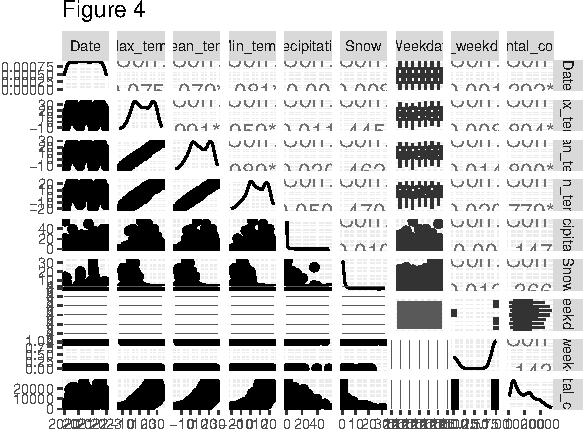
\includegraphics{Report_files/figure-latex/figure 4-1.pdf}

From Figure 4, note that the ``Rental\_count'', ``Precipitation'', and
``Snow'' are all severely right skewed, as noted before. Also notice
significant levels of correlation between the ``Rental\_count'' and all
variables. More in depth investigation would need to be conducted to
determine the exact nature of the relationship (linear, periodic, etc).

There is also significant correlation between the minimum, mean, and
maximum temperatures (which is expected), so perhaps if we were to fit a
model we would only want to select one of the temperature variables.
Also notice the periodic relationship between temperature and date.

There is also a significant imbalance in the ``is\_Weekday'' variable,
which is expected, as there are more weekdays than weekends in a year.
This is something to note as it may skew any results concerning this
variable.

A further point of interest is the scatter plot between
``Precipitation'' and ``Snow'', where we notice a few outlier points
with both large amount of rain and large amounts of snow. This is
interesting, as rain and snow do not usually occur together in such
large amounts on the same day.

Additionally, there are so many data points that it is impossible to
tell the relationship between some pairs of variables using these
scatter plots. For example, between Weekday\_num and Date. This is
acceptable for our purposes, as we are not specifically interested in
the relationship between these variables, just if there are any major
issues that could affect our ability to answer the question of interest.
However, in the future it may be necessary to redo the plots with
perhaps a subset of the data if we desire to model these relationships.

\hypertarget{preliminary-results}{%
\subsection{Preliminary Results}\label{preliminary-results}}

\hypertarget{maximum-and-minimum-rental-days}{%
\subsubsection{Maximum and Minimum Rental
Days}\label{maximum-and-minimum-rental-days}}

\begin{table}[!h]

\caption{\label{tab:Table 11 conditions for maximum bike share riders (all stations)}Table 11: Summary of top five days by rental count (all stations)}
\centering
\begin{tabular}[t]{l|r|r|r|r|r|r|l}
\hline
Date & Rental Count & Max Temperature (°C) & Min Temperature (°C) & Mean Temperature (°C) & Precipitation (mm) & Snow (cm) & Weekday\\
\hline
2022-08-13 & 27312 & 25.2 & 13.6 & 19.4 & 0.0 & 0 & Saturday\\
\hline
2022-08-20 & 26702 & 30.0 & 19.5 & 24.8 & 0.8 & 0 & Saturday\\
\hline
2022-08-27 & 26557 & 23.1 & 14.0 & 18.6 & 0.0 & 0 & Saturday\\
\hline
2022-09-10 & 26491 & 26.5 & 19.7 & 23.1 & 0.0 & 0 & Saturday\\
\hline
2022-07-16 & 26285 & 29.2 & 18.4 & 23.8 & 0.0 & 0 & Saturday\\
\hline
\end{tabular}
\end{table}

From Table 11, notice that all the days have a reasonable minimum and
maximum temperature (not too cold and not too hot), no (or very little)
rain, no snow, and most interestingly, all days are on a Saturday.
Furthermore, all 5 days are in 2022, and there are none in 2020 and
2021. This may be due to increase in ridership over time, or the COVID
situation in 2020 and 2021.

\begin{table}[!h]

\caption{\label{tab:Table 12 conditions for maximum bike share riders (most popular)}Table 12: Summary of top five days by rental count (most popular)}
\centering
\begin{tabular}[t]{l|r|r|r|r|r|r|l}
\hline
Date & Rental Count & Max Temperature (°C) & Min Temperature (°C) & Mean Temperature (°C) & Precipitation (mm) & Snow (cm) & Weekday\\
\hline
2021-06-06 & 456 & 30.5 & 18.9 & 24.7 & 0.0 & 0 & Sunday\\
\hline
2021-09-06 & 450 & 24.0 & 14.4 & 19.2 & 3.5 & 0 & Monday\\
\hline
2022-07-02 & 409 & 29.4 & 15.3 & 22.4 & 0.0 & 0 & Saturday\\
\hline
2022-05-14 & 403 & 27.0 & 16.6 & 21.8 & 0.0 & 0 & Saturday\\
\hline
2021-05-16 & 380 & 22.7 & 11.7 & 17.2 & 0.0 & 0 & Sunday\\
\hline
\end{tabular}
\end{table}

From Table 12, notice that similar to Table 11, all the days have a
reasonable minimum and maximum temperature (not too cold and not too
hot), no (or very little) rain, no snow. One difference is that the top
five days also includes Sundays, unlike Table 11, and also a Monday that
is not a holiday.

\begin{table}[!h]

\caption{\label{tab:Table 13 conditions for maximum bike share riders (median popular)}Table 13: Summary of top five days by rental count (median popularity)}
\centering
\begin{tabular}[t]{l|r|r|r|r|r|r|l}
\hline
Date & Rental Count & Max Temperature (°C) & Min Temperature (°C) & Mean Temperature (°C) & Precipitation (mm) & Snow (cm) & Weekday\\
\hline
2022-08-07 & 108 & 31.4 & 23.2 & 27.3 & 0 & 0 & Sunday\\
\hline
2022-08-13 & 103 & 25.2 & 13.6 & 19.4 & 0 & 0 & Saturday\\
\hline
2022-07-31 & 95 & 27.4 & 17.7 & 22.6 & 0 & 0 & Sunday\\
\hline
2022-08-06 & 94 & 30.5 & 21.7 & 26.1 & 0 & 0 & Saturday\\
\hline
2022-08-10 & 91 & 26.6 & 17.3 & 22.0 & 0 & 0 & Wednesday\\
\hline
\end{tabular}
\end{table}

In Table 13, again, similar to Table 11 and Table 12, all the days have
a reasonable minimum and maximum temperature (not too cold and not too
hot), no (or very little) rain, no snow. The most major difference is
that similar to Table 12, here we see a Wednesday (not a holiday or
weekend) included.

\begin{table}[!h]

\caption{\label{tab:Table 14 conditions for minimum bike share riders (all stations)}Table 14: Summary of bottom five days by rental count (all stations)}
\centering
\begin{tabular}[t]{l|r|r|r|r|r|r|l}
\hline
Date & Rental Count & Max Temperature (°C) & Min Temperature (°C) & Mean Temperature (°C) & Precipitation (mm) & Snow (cm) & Weekday\\
\hline
2022-01-18 & 399 & 0.2 & -10.1 & -5.0 & 0.8 & 32 & Tuesday\\
\hline
2022-01-17 & 460 & -2.3 & -5.0 & -3.6 & 36.2 & 25 & Monday\\
\hline
2020-01-19 & 589 & 1.3 & -10.4 & -4.5 & 0.3 & 14 & Sunday\\
\hline
2021-02-16 & 642 & -6.4 & -12.0 & -9.2 & 5.5 & 16 & Tuesday\\
\hline
2020-12-25 & 664 & 0.2 & -4.7 & -2.2 & 5.1 & 4 & Friday\\
\hline
\end{tabular}
\end{table}

From Table 14, notice that all days are very cold, and have some snow or
precipitation. The day of the week appears to have less effect here than
in Table 11, as there is a wide range here. Notice that these dates also
all occur in Dec-Feb winter months.

\begin{table}[!h]

\caption{\label{tab:Table 15 conditions for minimum bike share riders (most popular)}Table 15: Summary of bottom five days by rental count (most popular)}
\centering
\begin{tabular}[t]{l|r|r|r|r|r|r|l}
\hline
Date & Rental Count & Max Temperature (°C) & Min Temperature (°C) & Mean Temperature (°C) & Precipitation (mm) & Snow (cm) & Weekday\\
\hline
2020-02-02 & 2 & 2.5 & -0.1 & 1.2 & 6.1 & 4 & Sunday\\
\hline
2020-03-23 & 2 & 3.9 & 0.4 & 2.2 & 12.1 & 3 & Monday\\
\hline
2021-02-18 & 2 & -2.6 & -6.2 & -4.4 & 3.7 & 13 & Thursday\\
\hline
2022-01-26 & 3 & -8.6 & -14.0 & -11.3 & 0.1 & 24 & Wednesday\\
\hline
2020-12-25 & 3 & 0.2 & -4.7 & -2.2 & 5.1 & 4 & Friday\\
\hline
2020-01-12 & 3 & 2.2 & -5.2 & -1.5 & 12.8 & 2 & Sunday\\
\hline
\end{tabular}
\end{table}

From Table 15, notice that the minimum daily rental counts are very
small. Similar to Table 14, notice that all days are very cold, and
often have some snow or precipitation. The day of the week appears to
have less effect here than in Table 12, as there is a wide range here.

\begin{table}[!h]

\caption{\label{tab:Table 16 conditions for minimum bike share riders (median popularity)}Table 16: Summary of bottom five days by rental count (median popular)}
\centering
\begin{tabular}[t]{l|r|r|r|r|r|r|l}
\hline
Date & Rental Count & Max Temperature (°C) & Min Temperature (°C) & Mean Temperature (°C) & Precipitation (mm) & Snow (cm) & Weekday\\
\hline
2022-01-24 & 1 & -3.8 & -14.7 & -9.2 & 4.7 & 20 & Monday\\
\hline
2022-12-26 & 1 & -4.4 & -8.1 & -6.2 & 0.0 & 0 & Monday\\
\hline
2022-12-11 & 1 & -0.4 & -1.8 & -1.1 & 4.4 & 0 & Sunday\\
\hline
2022-01-22 & 1 & -3.8 & -12.4 & -8.1 & 0.0 & 22 & Saturday\\
\hline
2022-02-03 & 1 & -2.1 & -9.6 & -5.9 & 3.5 & 19 & Thursday\\
\hline
2022-01-20 & 1 & -7.3 & -16.4 & -11.9 & 0.0 & 24 & Thursday\\
\hline
2022-02-20 & 1 & 7.5 & -8.1 & -0.3 & 0.0 & 13 & Sunday\\
\hline
2021-12-25 & 1 & 7.4 & 3.3 & 5.4 & 4.8 & 0 & Saturday\\
\hline
2022-01-11 & 1 & -1.7 & -20.0 & -10.8 & 0.0 & 0 & Tuesday\\
\hline
2022-02-19 & 1 & -1.3 & -9.1 & -5.2 & 1.5 & 16 & Saturday\\
\hline
2021-12-27 & 1 & 1.3 & -5.3 & -2.0 & 1.9 & 0 & Monday\\
\hline
2022-12-25 & 1 & -3.9 & -8.6 & -6.2 & 0.0 & 1 & Sunday\\
\hline
\end{tabular}
\end{table}

From Table 16, notice that the minimum daily rental counts are all ones.
Recall from previous data exploration that the days with no rental
counts are not included here, so it is very likely that there are many
days with no rental counts that is not in this table. Aside from that,
similar to Table 14 and Table 15, notice that all days are very cold,
and often have some snow or precipitation. The day of the week appears
to have less effect here than in Table 13, as there is a wide range
here. Notice that these dates also all occur in Dec-Feb winter months.

From these six tables (11-16), observe that the general relationship
between bike share ridership and temporal and weather factors is very
similar even when we consider stations separately, so there is likely no
unique pattern of ridership count for each station. Thus, below, we will
only consider the total daily counts of bike rentals, not the individual
counts for the most popular and median popular station.

\hypertarget{rental-count-associations}{%
\subsubsection{Rental Count
Associations}\label{rental-count-associations}}

Figure 5, which shows the Rental count vs Temperature, can be found on
the website labelled Figure 5 in the Results section.

In Figure 5, notice that the trend appears to be relatively similar for
mean, max, and min temperatures. Also notice large fluctuations in
rental count as the temperature increases, indicating that much of the
variation in the rental count is still not explained by the temperature.
However, there is a clear trend that increase in temperature increases
rental count, at least up to a certain point. Once max temperature is
too high (roughly above 30°C), then the rental count starts to fall
again. Also notice that as the temperature increases, the variation in
rental count also increases.

\begin{center}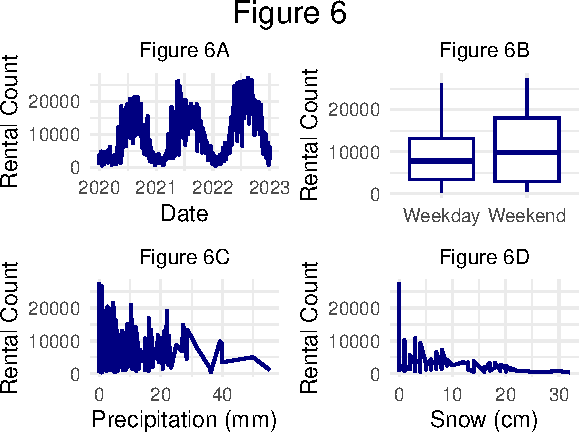
\includegraphics{Report_files/figure-latex/unnamed-chunk-15-1} \end{center}

In figure 6A, notice the clear trend of increasing ridership count in
the summer months, then decreasing ridership count in the winter months.
Also note that date and temperature are correlated, so the relationship
seen here could be a reflection of the relationship seen in Figure 5.
Again note the large variations in rental count across the dates. For
example, in the middle of 2022, there are a few very large dips in the
rental count. Also note how the variation in rental count is higher in
the summer months than in winter months.

From Figure 6B, notice that the median of the rental counts for the
weekday and weekend are actually relatively similar (differing by about
1500) whereas the third quantile differs greatly (by about 5000),
indicating that there tends to be a higher rental count more often on
the weekend. Recall from Figure 5 and 6A how when the temperature is
lower (i.e.~in the winter months), there is less variation in the rental
counts, and there is also lower rental count. This is reflected here in
Figure 6B, where being on the weekend or not has less impact on the
rental count when the rental count is low. Perhaps being on the weekend
or not instead explains the variation in rental counts when the
temperature is high (i.e.~in the summer months).

From Figure 6C, notice that when precipitation is low, there is very
large variation in rental count, however when the precipitation
increases, the rental count also tends to decrease somewhat. Do note
that there are not many data points with more than 30 mm of
precipitation, so trends seen may not be generalizeable. Also note that
rain does not tend to fall in the colder winter months, where there is
less bike ridership (as seen in Figure 5 and Figure 6A).

From Figure 6D, first notice that for nonzero values of snow, the
variation in rental count is not very large, especially as the amount of
snow increases. Do note that there is not a lot of nonzero data on snow,
so this may not be generalizeable. However, from the data that we do
have, even a little amount of snow appears to cap the rental count at
12000 per day. Also note that snow is correlated with temperature, in
that it generally only appears in the cold winter months, where there is
less bike ridership (as seen in Figure 5 and Figure 6A).

Some lingering issues with Figure 6C and Figure 6D is that the
precipitation and snow is recorded for the entire day, and it is unknown
whether this occurred late at night and/or for a very short amount of
time, resulting in less impact on ridership for that rainfall/snowfall.
To investigate this, hourly data would need to be used instead.

\hypertarget{rental-count-associations-with-day-of-week}{%
\subsubsection{Rental Count Associations with Day of
Week}\label{rental-count-associations-with-day-of-week}}

Now, let's take a look at the variables again, this time taking into
account the day of the week.

In the figures below, we will examine whether the relationship between
daily bike rental counts in Toronto and other weather variables is
influenced by the day of the week.

Figure 7 (Rental Count vs Mean Temp with Weekday), Figure 8 (Rental
Count vs Precipitation with Weekday), Figure 9 (Rental count vs Snow
with Weekday) can be found on the website under the Results section.

From Figure 8 and 9, we can observe that the day of the week doesn't
seem to change the relationship between precipitation and bike ridership
and snow and bike ridership. On the other hand, in Figure 7, there does
appear to be a slight tendency toward more bike share ridership on
weekends versus weekdays.

\hypertarget{effect-of-weather-interactions}{%
\subsubsection{Effect of Weather
Interactions}\label{effect-of-weather-interactions}}

Now we will explore whether interactions between weather variables
affects (e.g.~will rain on a warm or cold day be more likely to affect
rental count)

Figure 10 can be found on the website under the Results section.

In Figure 10, the larger the circle, the more precipitation there is.
Looking at the size of the circles, notice that when temperature is held
constant, the precipitation does decrease rental count, however having a
higher mean temperature means that even if there is precipitation, the
rental count is still higher than with a significantly lower mean
temperature and no precipitation.

\hypertarget{model}{%
\subsection{Model}\label{model}}

Now that we have looked more closely at the individual relationships
between the variables, let's try creating a model to quantify these
relationships. From previous analysis, we have discovered a cyclic
relationship, so the best model is likely to be a non-linear generalized
additive model (GAM). Specifically, we will add a cubic spline to the
Date variable, and include all other temporal and weather factors (only
Mean\_temp will be used for temperature, as we have already established
the three temperature variables provide the same information) as the
other predictors in the model.

Table 17:

\begin{table}[!h]
\centering
\begin{tabular}[t]{lcc}
\toprule
  & Full model & Reduced model\\
\midrule
(Intercept) & \num{8474.646} & \num{8468.749}\\
 & \num{<0.001}*** & \vphantom{3} \num{<0.001}***\\
Mean\_temp & \num{290.769} & \num{290.631}\\
 & \num{<0.001}*** & \vphantom{2} \num{<0.001}***\\
is\_weekday & \num{-2201.063} & \num{-2201.857}\\
 & \num{<0.001}*** & \vphantom{1} \num{<0.001}***\\
Precipitation & \num{-193.740} & \num{-194.146}\\
 & \num{<0.001}*** & \num{<0.001}***\\
Snow & \num{-6.358} & \\
 & \num{0.761} & \\
s(as.numeric(Date)) & \num{<0.001}*** & \num{<0.001}***\\
\midrule
Num.Obs. & \num{1088} & \num{1088}\\
R2 & \num{0.875} & \num{0.876}\\
AIC & \num{19998.4} & \num{19991.6}\\
BIC & \num{20073.2} & \num{20061.3}\\
RMSE & \num{2339.65} & \num{2334.40}\\
\bottomrule
\end{tabular}
\end{table}

Note that there is no estimate value for the spline on Date for the two
models, as the spline does not provide such an estimate. Instead, only
the p-value is provided next to \texttt{s(as.numeric(Date))} in the
bale. After fitting the full model, we observed that the predictor for
Snow is statistically insignificant, so we use the reduced model
instead.

Now all the predictors are statistically significant. Our final chosen
model (the reduced model) has response variable Rental\_count, and
predictors Mean\_temp, is\_weekday, Precipitation, and Date, where there
is a cubic spline on Date. We obtain that the adjusted R-squared value
is 0.876, indicating that about 87\% of the variation in the response
(Rental\_count) is explained by the predictors. This is a pretty large
percentage, so we can safely conclude that the total daily bike rental
counts is heavily influenced by weather factors of temperature and
precipitation, as well as temporal factors of the date and being a
weekend.

\hypertarget{conclusions}{%
\subsection{Conclusions}\label{conclusions}}

The question of interest is investigation on if weather factors and
temporal factors influence the number of bike share users on a given day
in Toronto. From the preliminary analysis of the data, we have gained
several insights.

First, from the tables we see that days with high ridership count tend
to have a comfortable temperature, be on a weekend or holiday, and have
no rain or snow. On the other hand, days with low ridership count tend
to be cold days (below 0°C), likely with precipitation or snow. This
pattern holds true for both the total daily rental count, and the daily
rental count for the most popular and median popular stations.

Then, more generally, as the temperature increases, the ridership count
increases, and the variation in the ridership count also increases.
Furthermore, in the summer months the ridership count increases (and has
higher variation), and in the winter months the ridership count
decreases (and has lower variation). Lower ridership counts appear
evenly spread between weekdays and weekends, but higher ridership counts
occur more often in weekends. In addition, both the occurrence of snow
and/or precipitation (that is, a nonzero value), tends to decrease the
ridership count.

Taking into account the day of week, we further discover that the day of
the week doesn't seem to change the relationship between precipitation
and bike ridership and snow and bike ridership. On the other hand, there
does appear to be a slight tendency toward more bike share ridership on
weekends versus weekdays.

A further observation is that when temperature is held constant, the
precipitation does decrease rental count, however having a higher mean
temperature means that even if there is precipitation, the rental count
is still higher than with a significantly lower mean temperature and no
precipitation.

Finally, after fitting a model that provided an adjusted R-squared value
of 0.876, we further concluded that the total daily bike rental counts
is heavily influenced by temperature, precipitation, date, and being a
weekend.

In addition, notice that the relationships discussed above appear to
hold true even when we consider the bike rentals for an individual
station instead of the sum of all stations.

\hypertarget{limitations}{%
\subsection{Limitations}\label{limitations}}

Since the weather data used is daily weather data, this does not capture
any patterns within the day. For example, there may be both large
amounts of snow and a large bike rental count for some day if the snow
occurs late at night, after many people have already rented bikes
earlier that day. For the temperature variables, we also do not know
exactly when an extreme low or high temperature is (although we can make
inferences based on our own knowledge). Thus, there is an underlying
assumption that the weather variables are representative of the entire
day.

There is also an underlying assumption that the weather data we
collected from the Toronto weather station is representative of Toronto
as a whole, while that may not be the case. Bike Share Toronto has bike
stations over almost 200 \(km^2\). That is a very large area, and
weather conditions within the areas may also vary.

The analysis of whether the association between the temporal and weather
factors varies for each individual bike station was only conducted using
two individual stations, where Bike Share Toronto actually has hundreds
of stations. A more strict analysis would be to model all the stations
individually, and perhaps there are some unique stations that have a
different association with the temporal and weather factors. However, it
was not possible to conduct such a large analysis in this report, so
that is merely an idea for future exploration.

\end{document}
